\documentclass[ngerman,aspectratio=169]{beamer}
\usepackage[utf8]{luainputenc}
\usepackage[TS1,T1]{fontenc}
\usepackage{babel}
\usetheme[pagenum,navbar,ddc]{tud}
\usepackage{xcolor}
\usepackage{listings}
\usepackage{tikz}
\usepackage{multicol}
\usepackage[labelformat=empty,font=scriptsize]{caption}
\usepackage{marvosym}

\lstset{language=C}
\lstdefinestyle{mystyle}{
	language=C,
	basicstyle=\ttfamily\footnotesize,
	commentstyle=\color{commentgreen},
	keywordstyle=\color{code_orange},
	numberstyle=\tiny\color{code_gray},
	stringstyle=\color{code_purple},
	showstringspaces=false,
	breakatwhitespace=true,      
	prebreak=...,   
	breaklines=true,                      
	numbers=left,                    
	numbersep=5pt,  
	tabsize=1
}

\title{TUN/TAP-Geräte \protect\\\mdseries Übersicht, Funktionsweise und Implementierung im Linux-Kernel\strut}
\subtitle{Proseminar Rechnernetze}
\author{Lucas Waclawczyk}

\newcommand*\inmm[1]{\pgfmathsetmacro\inmmwert{#1 / 1mm}\inmmwert}
\makeatletter
\newcommand*\inpt[1]{\setlength\@tempdima{#1}\the\@tempdima}
\makeatother

\AtBeginSection[]{\partpage{\usebeamertemplate***{part page}}}
\begin{document}
	\mode<presentation>{\setbeamertemplate{tud background}[image/shaded]{Seminarraum.jpg}{0.7}}
	\maketitle
	
	\mode<presentation>{\setbeamertemplate{page number in footline}[frame][text and total]}
	\frame{\frametitle{Inhalt}\tableofcontents}
	
	\section{Übersicht}
	\subsection{Rückblick Network Interfaces}
	\begin{frame}{Rückblick Network Interfaces}
		\only<1-3,5->{
			\begin{multicols}{2}
				\begin{itemize}
					\setlength{\itemsep}{1em}
					\item Interface = Schnittstelle
					\item zwischen zwei Schichten im OSI-Modell
					\visible<3,5->{
						\item übernimmt Daten von Instanz eines {$ (n+1) $-Protokolls}
						\item stellt Daten für Instanz eines {$ (n) $-Protokolls} bereit
					}
					\visible<5->{
						\item muss nicht physisch sein\\
						\MVRightArrow \: Virtual Network Interface
					}
				\end{itemize}
					\only<1>{\hspace{-.5cm}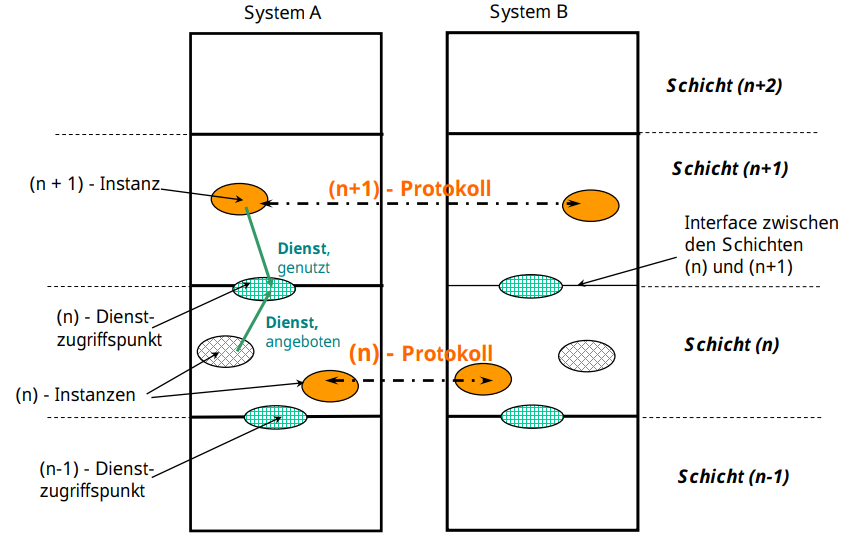
\includegraphics[width=1.2\linewidth]{network_interface}}
					\only<2,3,5->{\hspace{-.5cm}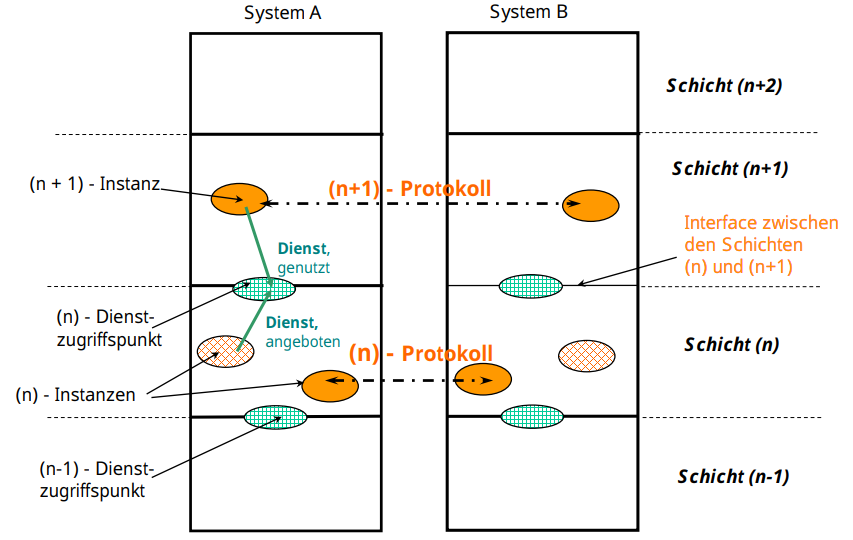
\includegraphics[width=1.2\linewidth]{network_interface_colored}}
					\centering aus \hyperlink{ref:rene}{[1]}
			\end{multicols}
		}
		\only<4>{
			\begin{figure}
				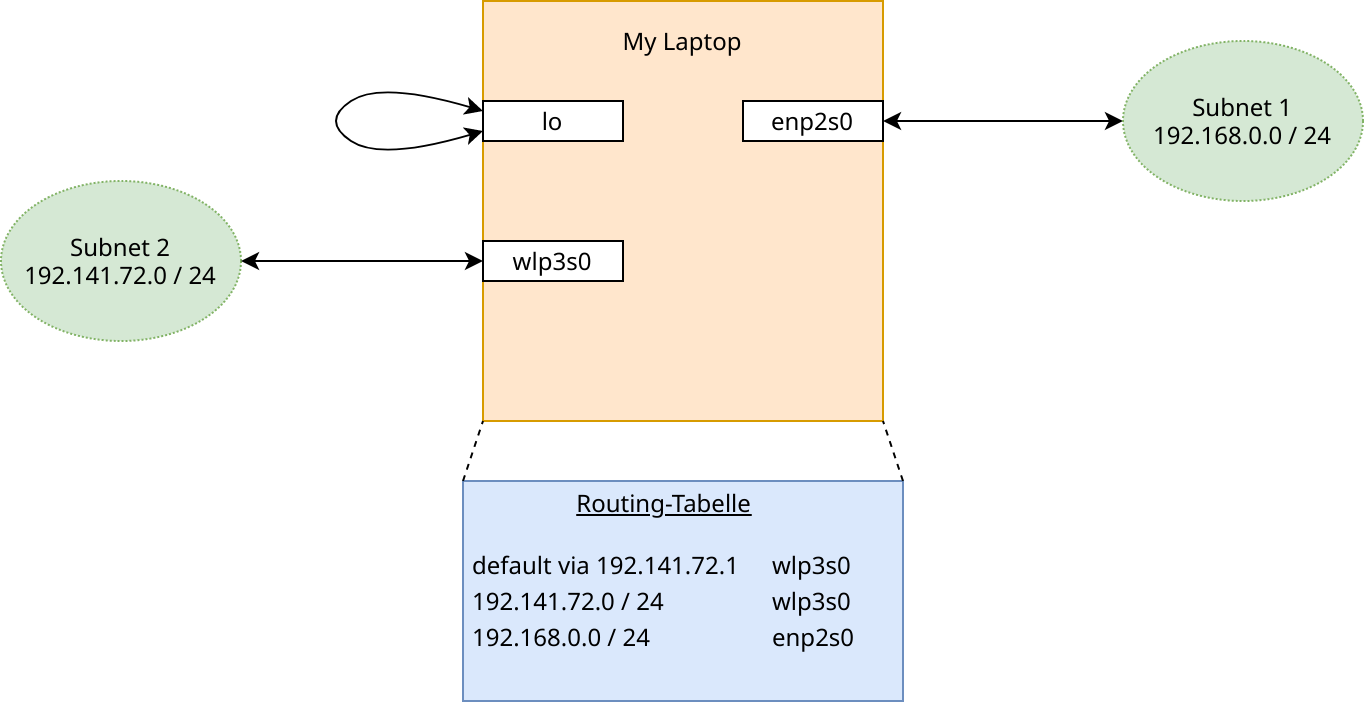
\includegraphics[width=.77\textwidth]{interfaces01}
				\caption{Network Interfaces relativ zu Gerät und Netz am Beispiel}
			\end{figure}
		}
	\end{frame}

	\subsection{Generelles zu TUN und TAP}
	\begin{frame}{Generelles zu TUN und TAP}
		\only<1,2,5->{
			\begin{itemize}
				\item Virtual Network Interfaces, d.h. man kann
				\begin{itemize}
					\item[\dots] ihnen IP-Adressen zuweisen
					\item[\dots] ihren Traffic analysieren
					\item[\dots] Firewall-Regeln für sie konfigurieren
					\item[\dots] uvm.
				\end{itemize}
				\visible<2,4->{
					\item \textit{Interface $ \leftrightarrow $ Anwendung} \:\: statt \:\: \textit{Interface $ \leftrightarrow $ physische Verbindung}
					\item nützlich für virtuelle Verbindungen
				}
				\visible<5->{
					\item u. A. Linux, Windows 2000 - 10, Mac OS X (nur TUN eingebaut)
					\item hier für Linux
				}
			\end{itemize}
		}
		\only<3>{
			\begin{figure}
				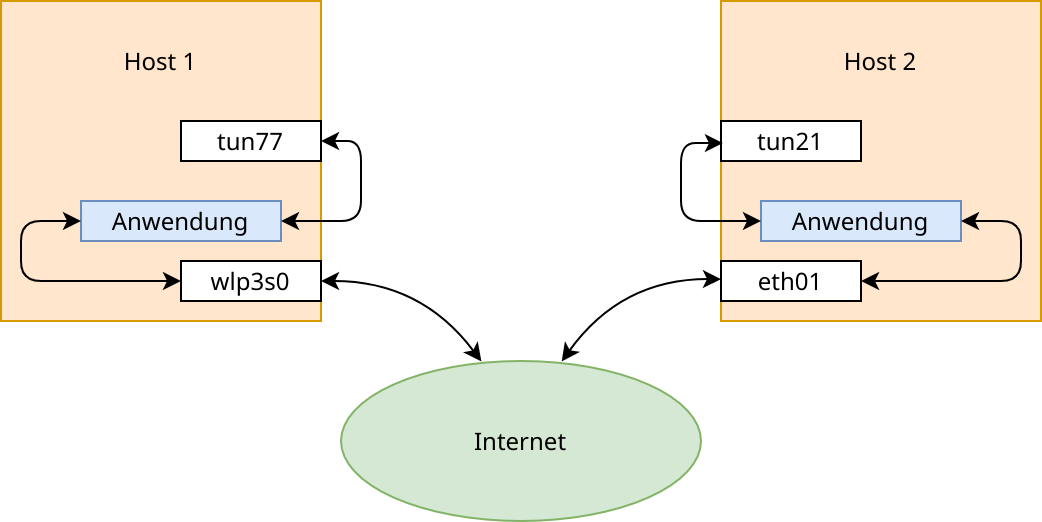
\includegraphics[width=.8\linewidth]{connection_physical}
				\caption{Schema einer virtuellen Verbindung (physische Ansicht)}
			\end{figure}
		}
		\only<4>{
			\begin{figure}
				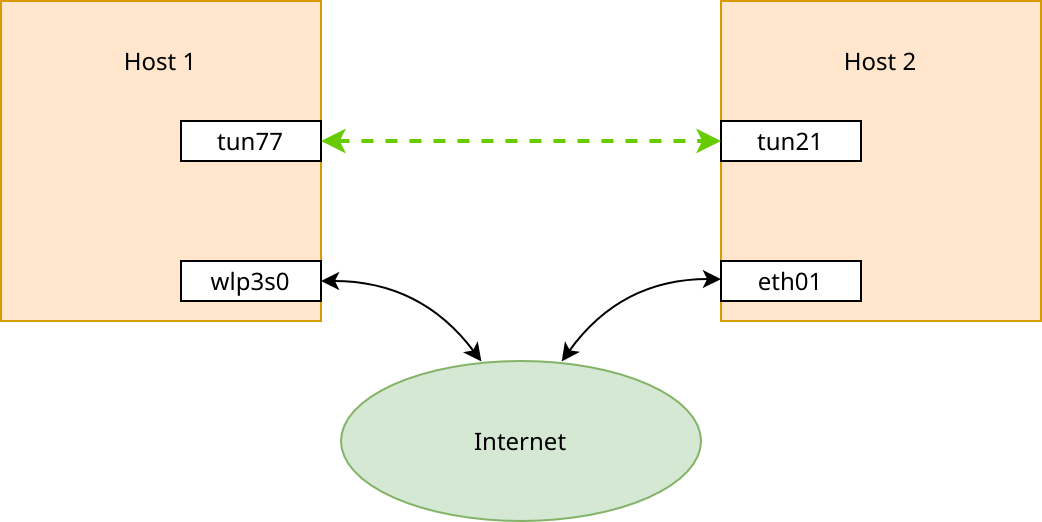
\includegraphics[width=.8\linewidth]{connection_virtual}
				\caption{Schema einer virtuellen Verbindung (virtuelle Ansicht)}
			\end{figure}
		}
	\end{frame}

	\subsection{TUN vs. TAP}
	\begin{frame}{TUN vs. TAP \hyperlink{ref:openvpn}{[7]}}
		\only<1,4,5,8,9>{
			\begin{multicols*}{2}
				\textbf{TAP --  Terminal Access Point}\\
				$ \sim $ Ethernet $ \sim $ Layer 2
				\begin{itemize}
					\visible<4->{
						\item[$ \oplus $] verhält sich wie echter Netzwerkadapter
						\item[$ \oplus $] flexible Protokollwahl
						\item[$ \oplus $] Bridging möglich
					}
					\visible<5->{
						\item[$ \ominus $] viel Overhead (Ethernet-Header, Broadcast)
						\item[$ \ominus $] skaliert schlecht
						\item[$ \ominus $] kein Support bei Android, iOS
					}
				\vspace{3cm}
			
				\textbf{TUN -- Netzwerk-Tunnel}\\
				$ \sim $ IP $ \sim $ Layer 3
				\begin{itemize}
					\visible<8->{
						\item[$ \oplus $] weniger Overhead (kein Ethernet-Header, kein Broadcast)
						\item[$ \oplus $] nur Layer-3-Pakete
					}
					\visible<9->{
						\item[$ \ominus $] nur Layer-3-Pakete
						\item[$ \ominus $] keine Broadcasts
						\item[$ \ominus $] kein Bridging möglich
					}
				\end{itemize}
				\end{itemize}
			\end{multicols*}
		}
		\only<2>{
			\begin{figure}
				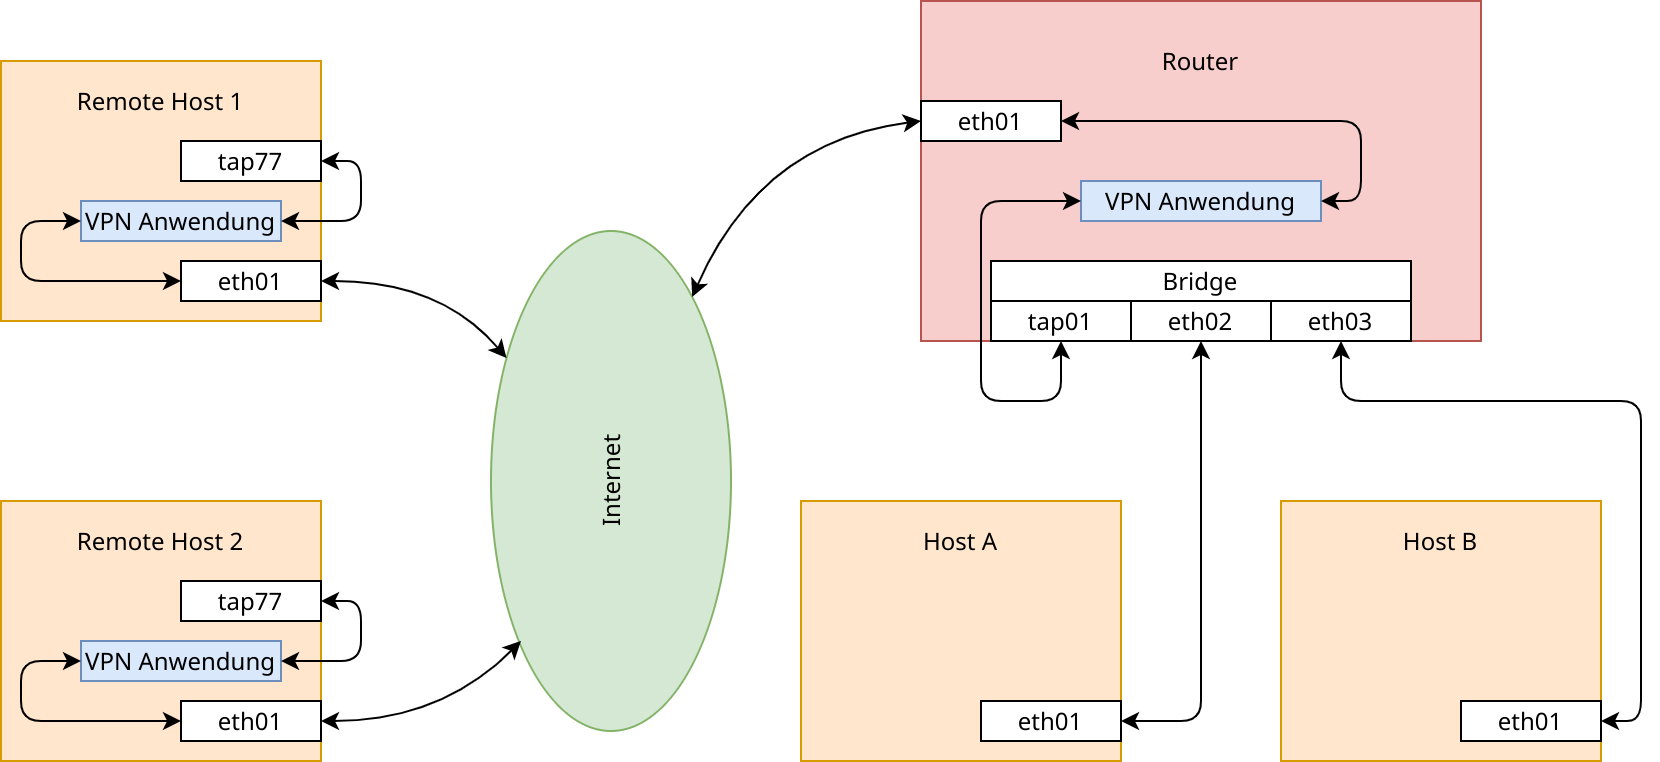
\includegraphics[width=.9\linewidth]{tap_physical}
				\caption{Anwendungsbeispiel TAP (physische Ansicht)}
			\end{figure}
		}
		\only<3>{
			\begin{figure}
				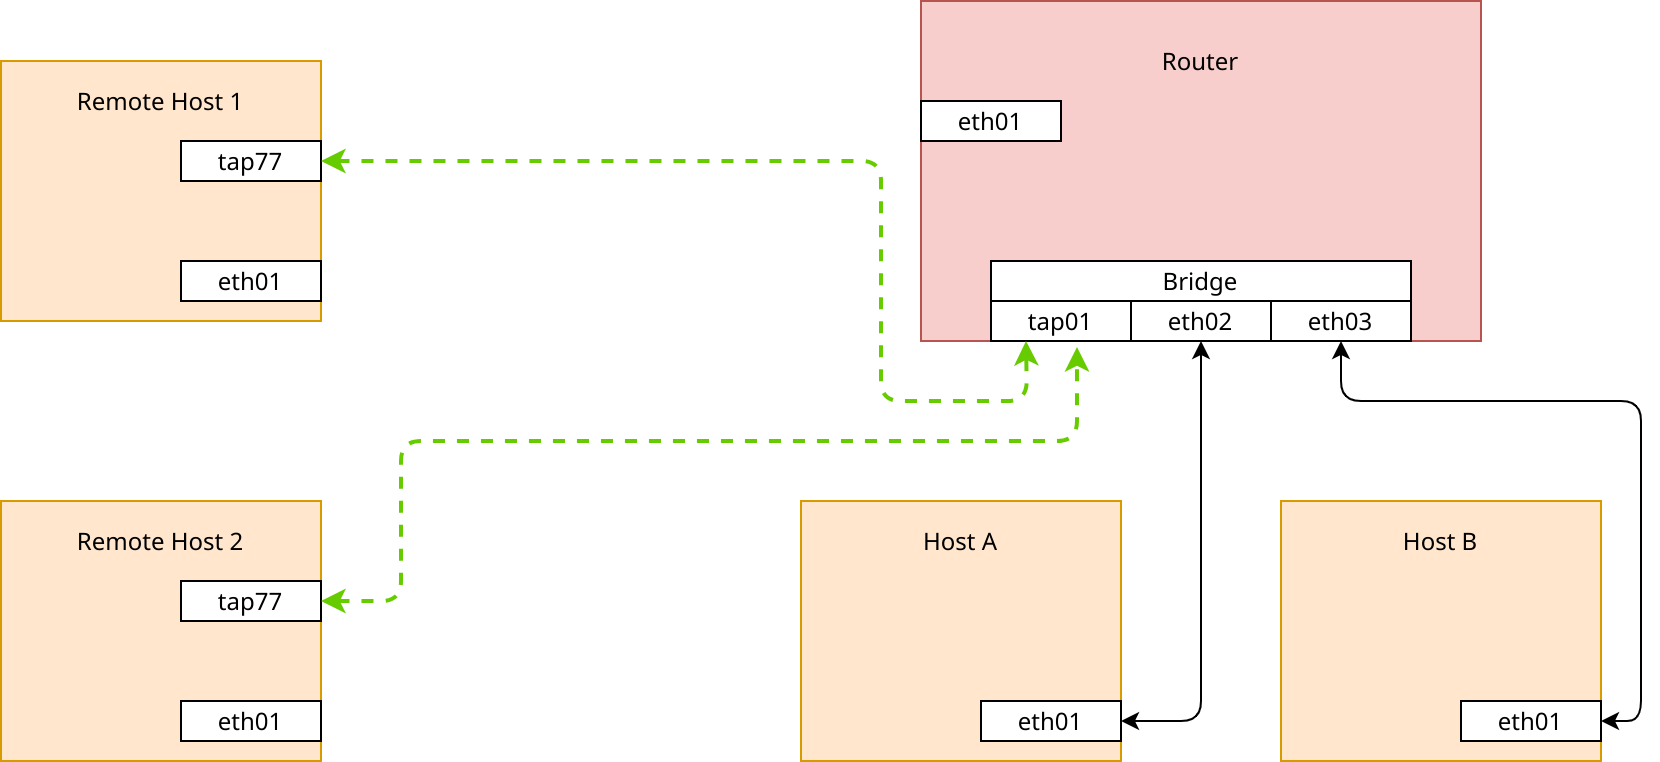
\includegraphics[width=.9\linewidth]{tap_virtual}
				\caption{Anwendungsbeispiel TAP (virtuelle Ansicht)}
			\end{figure}
		}
		\only<6>{
			\begin{figure}
				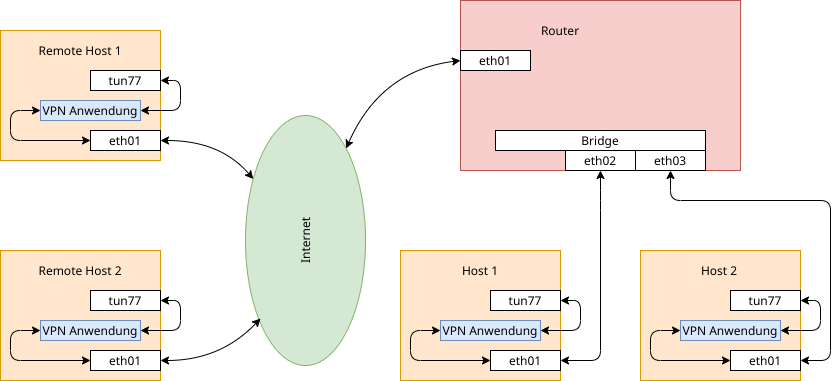
\includegraphics[width=.9\linewidth]{tun_physical}
				\caption{Anwendungsbeispiel TUN (physische Ansicht)}
			\end{figure}
		}
		\only<7>{
			\begin{figure}
				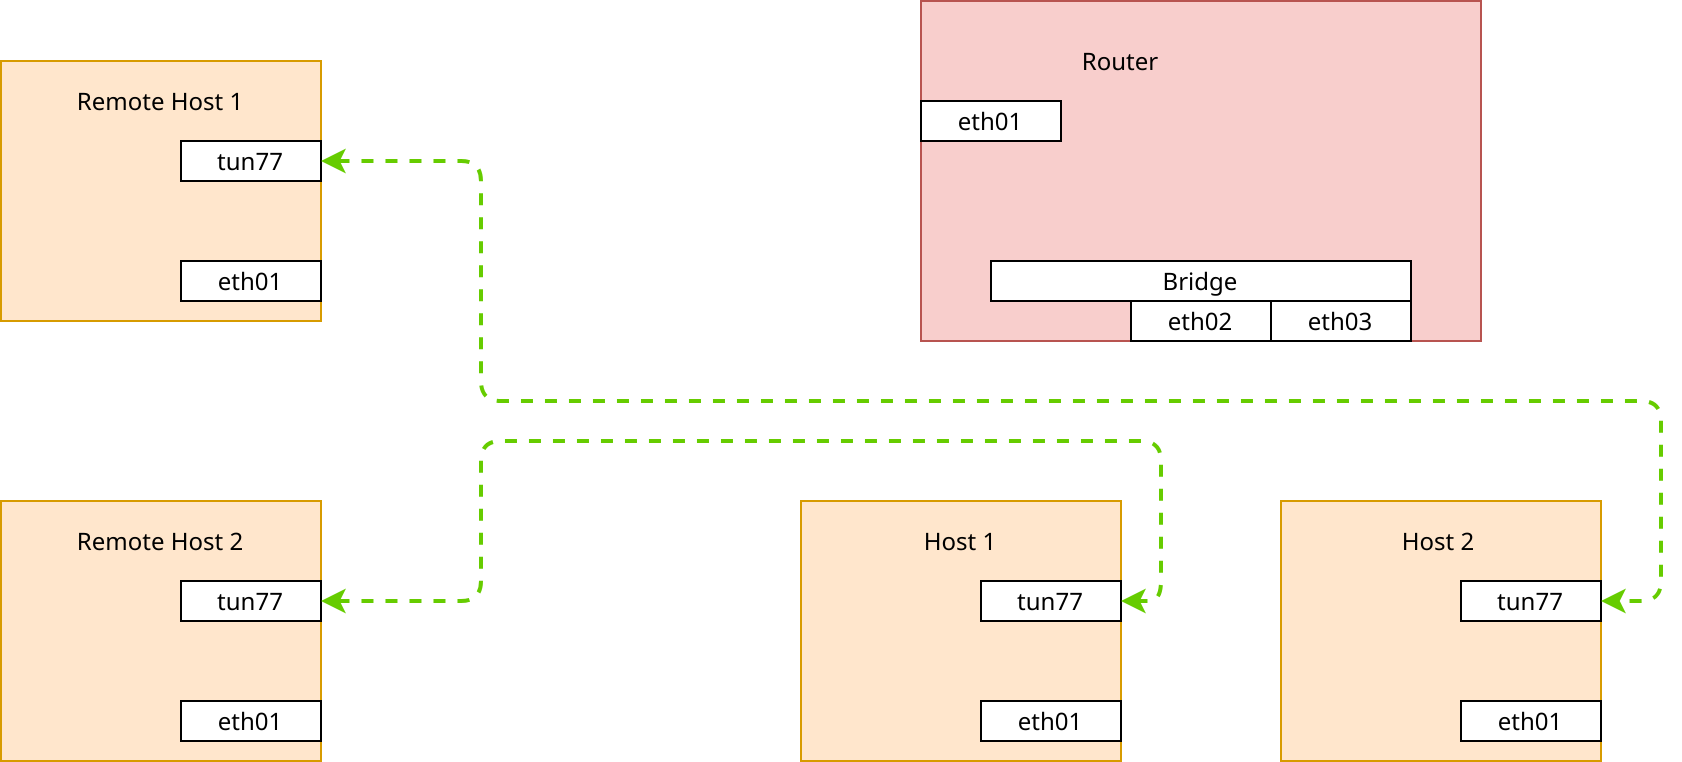
\includegraphics[width=.9\linewidth]{tun_virtual}
				\caption{Anwendungsbeispiel TUN (virtuelle Ansicht)}
			\end{figure}
		}
	\end{frame}

	\section{Implementierung in Linux}
	\subsection{Wichtige Adressen}
	\begin{frame}{Wichtige Adressen}
		\begin{itemize}
			\setlength\itemsep{.3cm}
			\item Kernel-Code:\\
			\url{https://github.com/torvalds/linux.git}
			
			\item TUN / TAP (Driver):\\
			\texttt{/linux/drivers/net/tun.c}
			
			\item Clone Device:\\
			\texttt{/dev/net/tun}
			
			\item diese Präsentation und Code:\\
			\url{https://github.com/lucaswzyk/pres_tun_tap.git}
		\end{itemize}
	\end{frame}
	
	\subsection{Aufbau -- Nutzung -- Abbau}
	\begin{frame}{Aufbau}
		\only<1,6>{
			Aufbau eines Interfaces (erfordert CAP\_NET\_ADMIN capability):
			\vspace{.3cm}
			\begin{enumerate}
				\setlength\itemsep{.3cm}
				\item öffne \texttt{/dev/net/tun} (Clone Device) mit Lese-Schreibberechtigung
				\item rufe syscall \texttt{ioctl(fd, TUNSETIFF, if\_req\_struct)} auf
				\visible<6>{
					\item persistiere Gerät (ggf.)
					\item weise IP-Adresse(n) zu
				}
			\end{enumerate}
		}
		\only<2>{
			\begin{figure}
				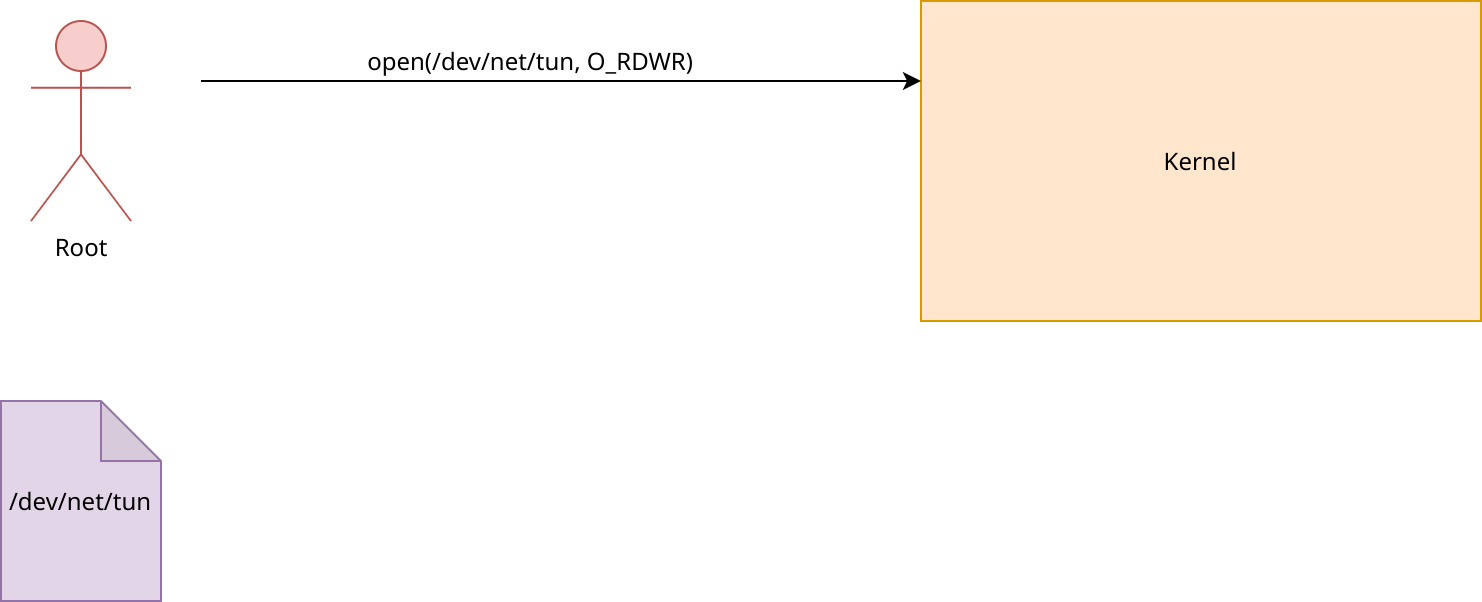
\includegraphics[width=\textwidth]{open_tun01}
				\caption{Aufbau eines Virtual Network Interfaces (1 / 4)}
			\end{figure}
		}
		\only<3>{
			\begin{figure}
				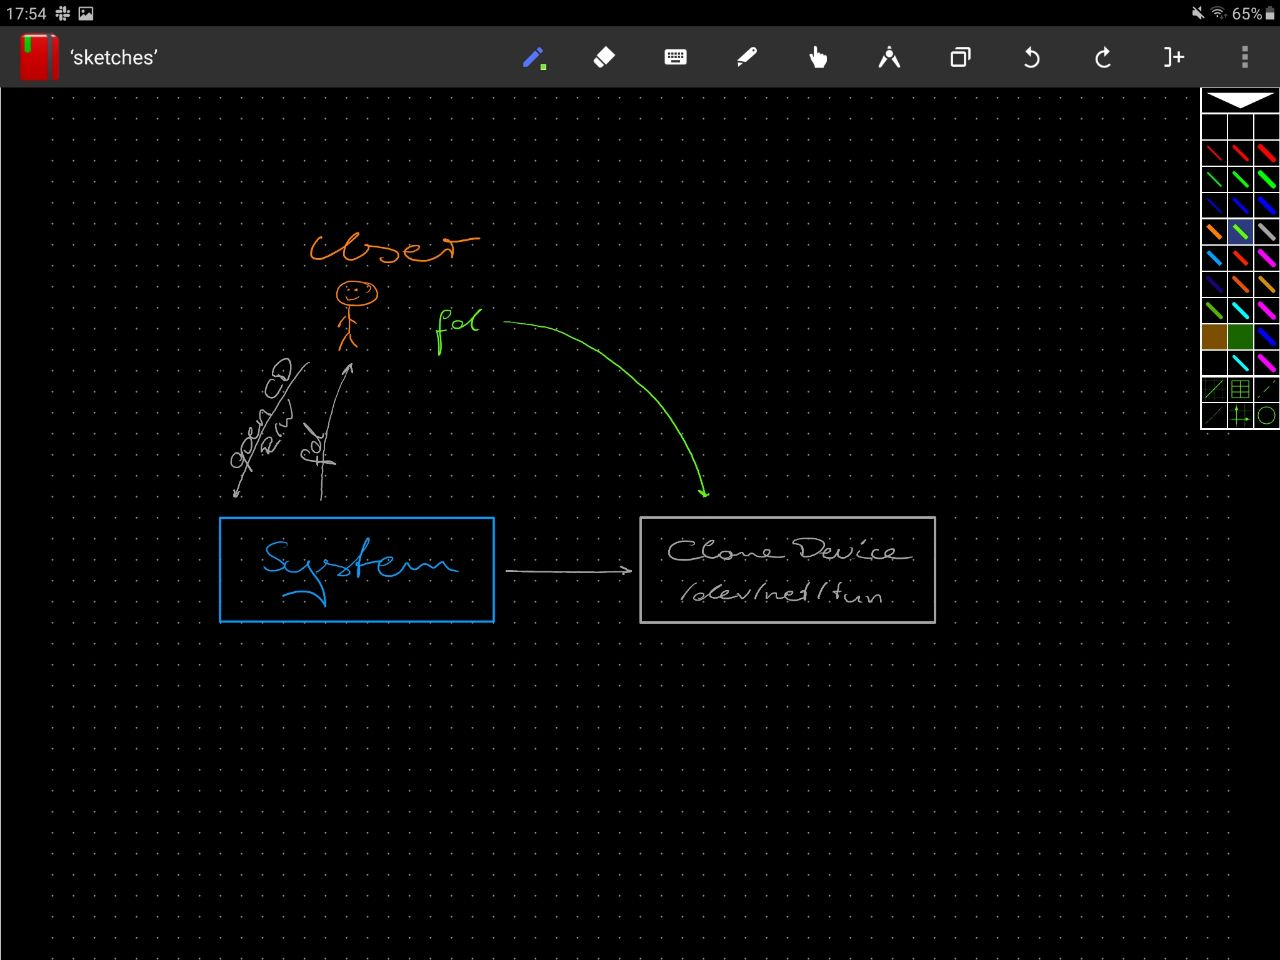
\includegraphics[width=\textwidth]{open_tun02}
				\caption{Aufbau eines Virtual Network Interfaces (2 / 4)}
			\end{figure}
		}
		\only<4>{
			\begin{figure}
				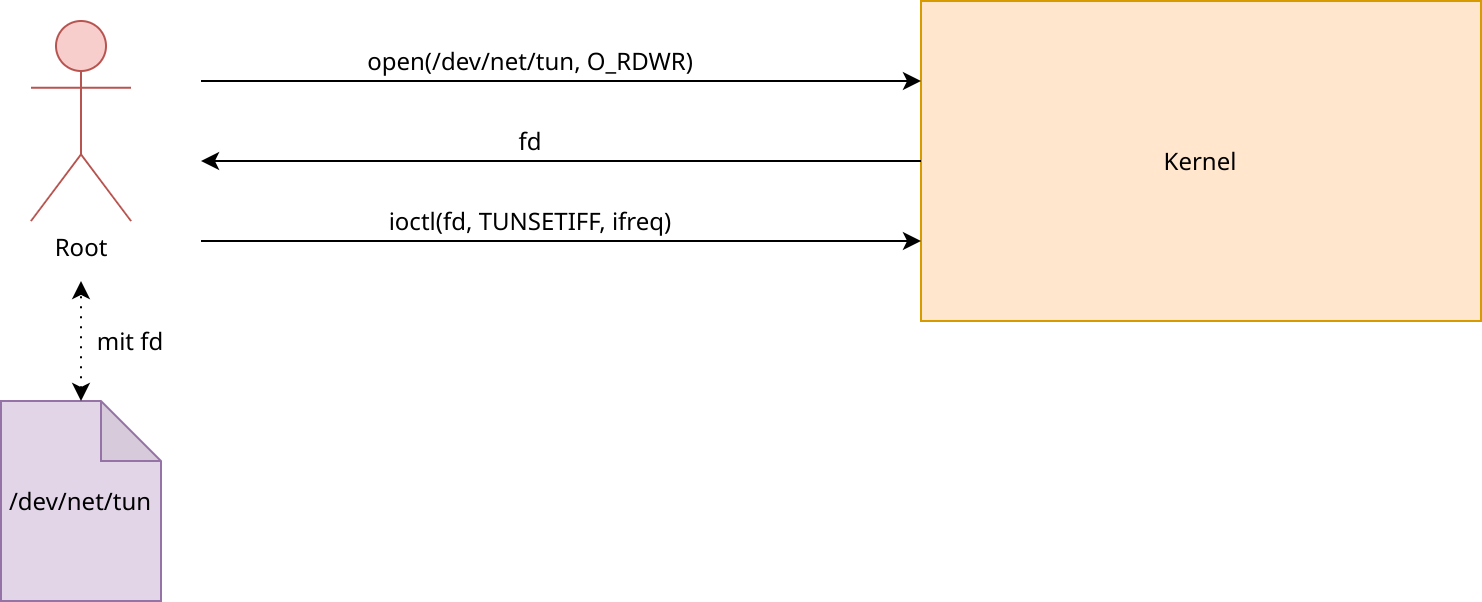
\includegraphics[width=\textwidth]{open_tun03}
				\caption{Aufbau eines Virtual Network Interfaces (3 / 4)}
			\end{figure}
		}
		\only<5>{
			\begin{figure}
				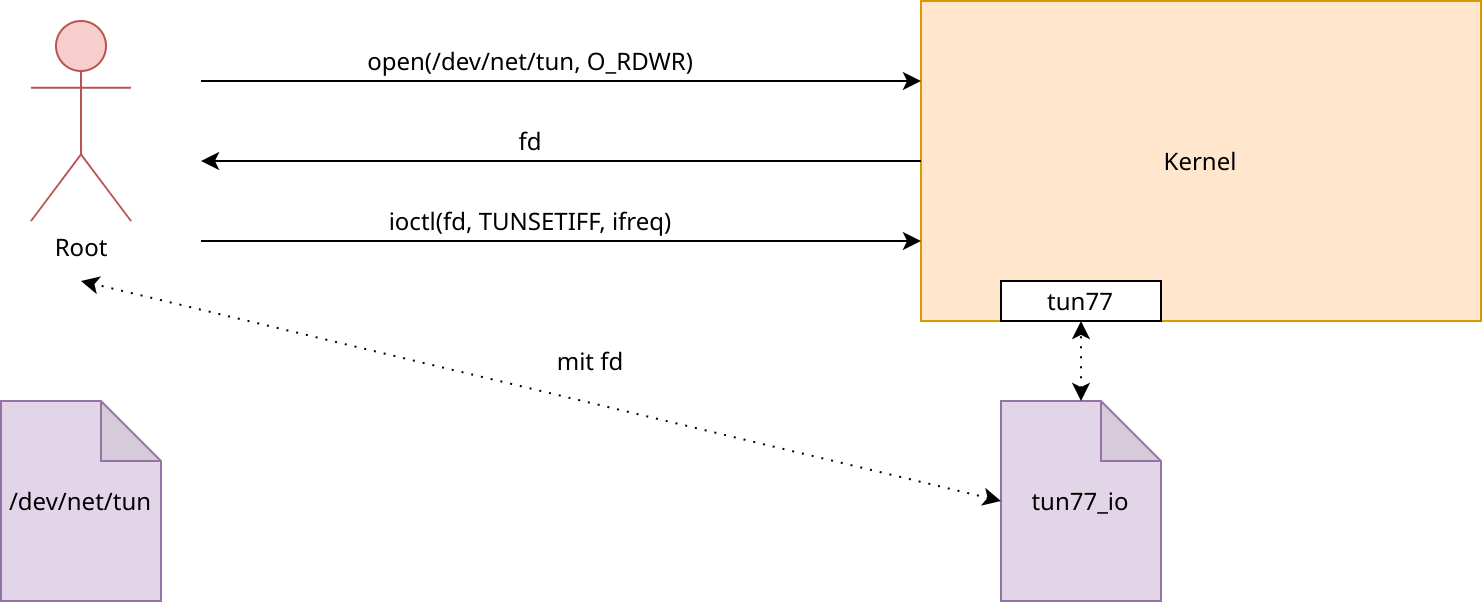
\includegraphics[width=\textwidth]{open_tun04}
				\caption{Aufbau eines Virtual Network Interfaces (4 / 4)}
			\end{figure}
		}
	\end{frame}

	\begin{frame}{Nutzung und Abbau}
		\only<1,3>{
			Nutzung:
			
			\begin{itemize}
				\item binde Anwendung an Interface
				\begin{itemize}
					\item wiederhole obiges als beliebiger Nutzer
					\item nutze bestehenden Interface-Namen
				\end{itemize}
				\item Lesen und Schreiben mittels \texttt{fd}
			\end{itemize}
			\vspace{.5cm}
			
			\visible<3>{
				Abbau:
				
				\begin{itemize}
					\item transientes Gerät verschwindet mit Beenden des Erzeuger-Prozesses
					\item persisitentes Gerät muss aktiv abgebaut werden (syscall)
				\end{itemize}
			}
		}
		\only<2>{
			\begin{figure}
				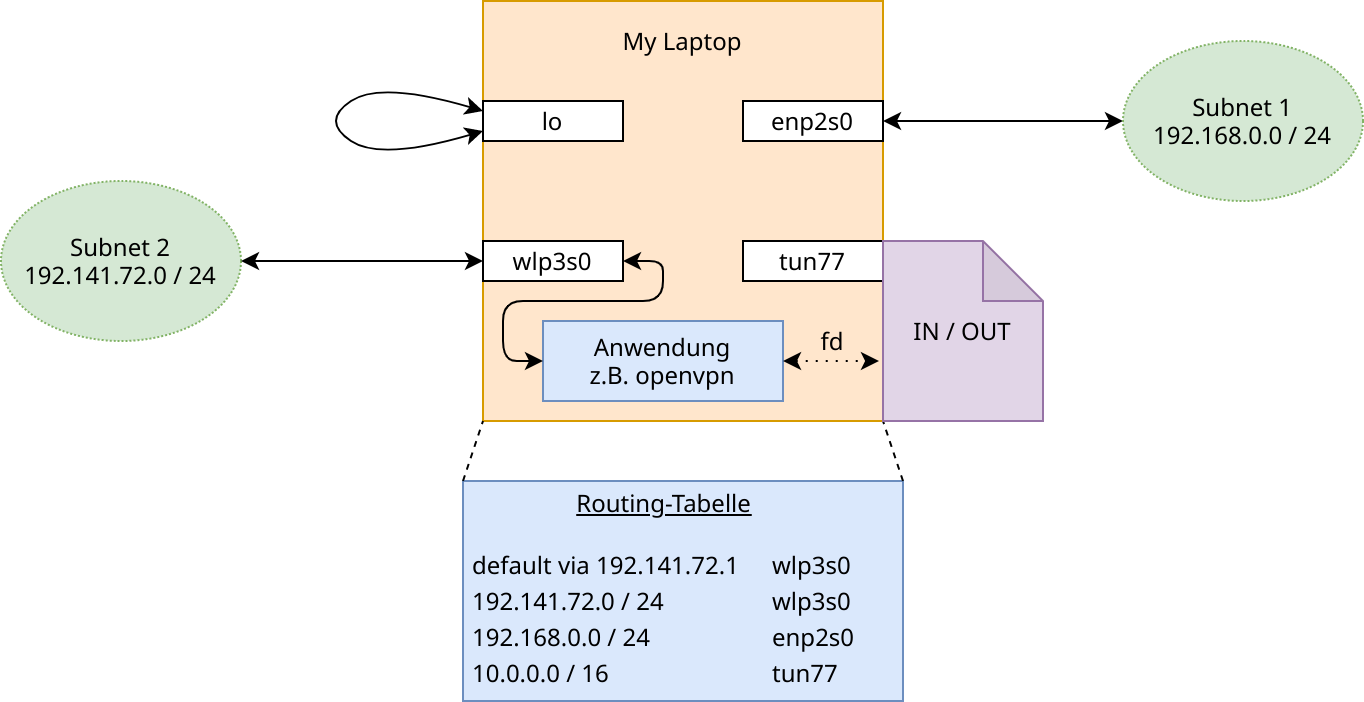
\includegraphics[width=.77\textwidth]{interfaces02}
				\caption{Network Interfaces (physisch und virtuell) relativ zu Gerät und Netz am Beispiel}
			\end{figure}
		}
	\end{frame}

	\subsection{Umsetzung als Structs}
	\begin{frame}[fragile]{Umsetzung als Structs}
		Auszug aus \texttt{/linux/drivers/net/tun.c}:
		
		\hspace{-5cm}
		\begin{minipage}{\textwidth}
			\begin{lstlisting}
			struct tun_struct {
				struct tun_file __rcu *tfiles[MAX_TAP_QUEUES];
				unsigned int flags;
				kuid_t owner;
				kuid_t group;
				struct net_device *dev;
			}
			
			struct tun_file {
				struct tun_struct __rcu *tun;
			}
			\end{lstlisting}
		\end{minipage}
	\end{frame}

	\section{Quellen}
	\begin{frame}{Quellen}
		\begin{enumerate}
			\item[{[1]}] Skript und Übungsaufgaben der Vorlesung Rechnernetze, TU Dresden 2019 (präzise genug?) \label{ref:rene}
			\item[{[2]}] \url{https://backreference.org/2010/03/26/tuntap-interface-tutorial/}
			\item[{[3]}] \url{https://www.elektronik-kompendium.de/sites/net/0811011.htm}
			\item[{[4]}] \url{https://en.wikipedia.org/wiki/TUN/TAP}
			\item[{[5]}] \url{https://www.thomas-krenn.com/de/wiki/OpenVPN_Grundlagen}
			\item[{[6]}] \url{https://floating.io/2016/05/tuntap-demystified/3/}
			\item [{[7]}] \url{https://community.openvpn.net/openvpn/wiki/BridgingAndRouting} \label{ref:openvpn}
		\end{enumerate}
\end{frame}
\end{document}
